\apendice{Plan de Proyecto Software}

\section{Introducción}
El plan de proyecto software relaciona todo aquello referido a la gestión del proyecto. Es un proceso muy importante para realizar antes de comenzar a trabajar en el desarrollo. En este punto, se llevan a cabo cosas como la planificación de tiempos para realizar las tareas, se definen los costes económicos del proyecto o l,a forma de trabajo.

Veremos dentro de la planificación temporal la manera en la que el trabajo y sus cargas han sido repartidas a lo largo de este tiempo desarrollando el proyecto. Todo esto tras haber analizado tanto el número de tareas a realizar, como la naturaleza de todas estas. 

Por otra parte, a través del estudio de viabilidad podremos poner la vista en las partes ecnómicas del proyecto. Analizaremos los costes derivados del proyecto y la gestión de las licencias utilizadas.

Podremos encontrar dos partes diferenciadas dentro de ese apartado:
\begin{itemize}
    \item Estudio de la viabilidad económica: Costes del proyecto dividiendo y analizando tanto en hardware, software como en personal.
    \item Estudio de la viabilidad legal: Análisis de las licencias para el uso de software especializado en el proyecto.
\end{itemize}

\section{Planificación temporal}
Como se comenta dentro de la memoria de este proyecto, la manera de trabajar y la metodología utilizada es la de SCRUM\cite{SCRUM} dentro del marco de las metodologías ágiles de desarrollo de software. Planificando dividiendo el tiempo en sprints que han de cubrirse en el tiempo marcado, con revisiones periódicas del trabajo.

Dentro de esto podemos ver que las 300 horas asignadas desde la Universidad de Burgos e ITCL\cite{itcl} han sido divididas en un total de seis sprints, cuya duración son de un total de dos semanas en todos los casos. 

Además, comentar que podríamos considerar como un sprint previo al trabajo la primera semana donde se realizó la toma de decisiones en referencia a lo que se iba a hacer, planificación de tareas y la metodología a seguir en cuanto a la forma de trabajar. También vimos que repositorios utilizaríamos, herramientas para la gestión o el control de versiones.  
\subsection{\textbf{Sprint 1 (07/03/2022-18/03/2022)}}
En este primer sprint se llevaron a cabo las instalaciones de aquellos softwares necesarios para el correcto desarrollo de esta parte del trabajo. También se establecieron unos puntos a cumplir relacionados en primer lugar con el 'aterrizaje' en el proyecto y en segundo lugar con el aprendizaje relativo a los guantes hápticos Nova \cite{SGloveNova}.

Las tareas dispuestas a cumplir son:
\begin{itemize}
    \item Continuar con el estudio de algunos aspectos de Unity\cite{Unity}.
    \item Estudio documentación relativa a los guantes y su SDK.
    \item Monitorizar y parametrizar lo que ofrecen los guantes.
    \item Desarrollo script que recoja datos de los guantes y aplique fuerzas hápticas\cite{Haptica1} o vibraciones.
    \item Desarrollo escena de representación 3D con \begin{enumerate}
        \item Paneles que controlen las fuerzas y vibraciones.
        \item Paneles que muestren datos de los sensores.
    \end{enumerate}
\end{itemize}

El desarrollo de este primer sprint se saldó de manera correcta sirviendo así para poder adaptarme fácilmente al proyecto y la empresa.


\newpage
\begin{figure}[t]
\centering
\label{Cierre de tareas del SPRINT 1}
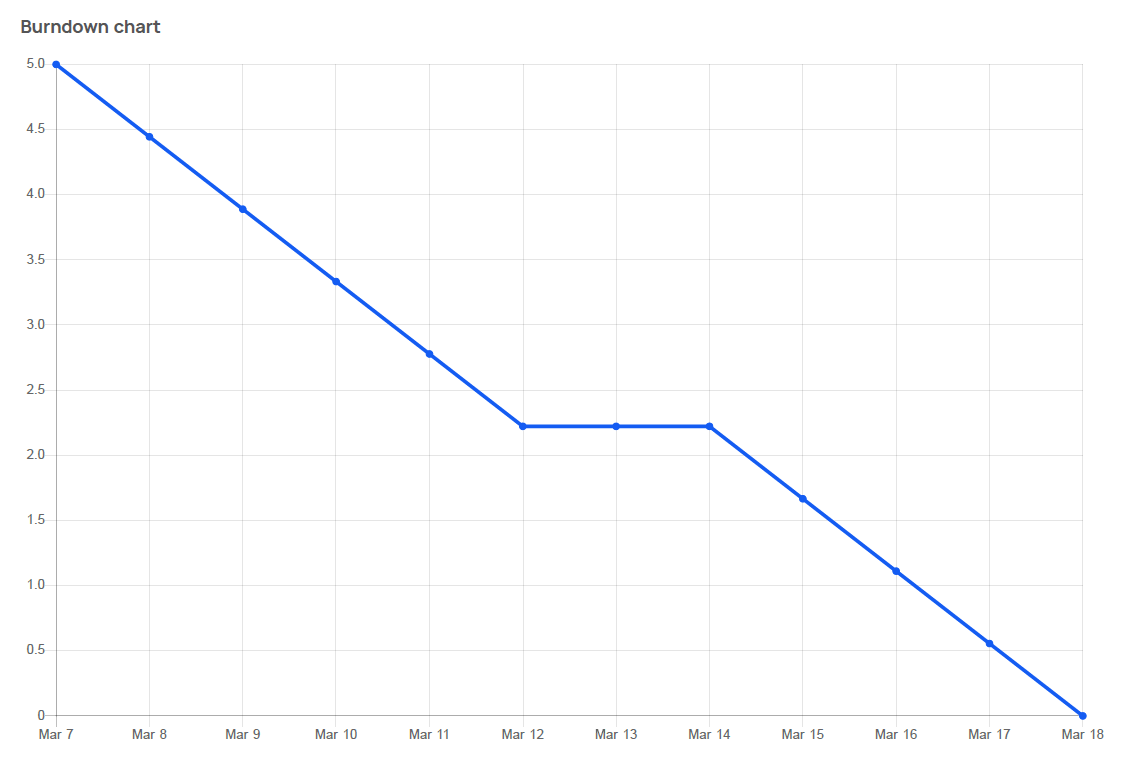
\includegraphics[width=0.6\textwidth]{img/sprint1.PNG}
\caption{Cierre de tareas del SPRINT 1}
\end{figure}

\subsection{\textbf{Sprint 2 (21/03/2022-01/04/2022)}}
En este segundo sprint los objetivos iban encaminados a mezclar por primera vez tanto el dispositivo Oculus Quest 2\cite{Quest2} y los guantes Nova. Se llevó a cabo la instalación del software de Oculus y llevamos a cabo la primera conexión. Se realizaron pruebas con ellas.

Para dar por correcta esta fusión de ambas partes teníamos las siguientes tareas:
\begin{itemize}
    \item Estudio de la componente\cite{Componentes} Transform de Unity, enfatizando en la posición.
    \item Análisis de las posibilidades de seguimiento (tracking) de Oculus.
    \item Sincronización de la vista en el mundo virtual con la visión de las gafas.
    \item Crear una escena con la adaptación de la primera escena a la realidad virtual.
    \item Cambiar el panel de fuerzas por uno que muestre datos de seguimiento.
    \item Representación tridimensional de la mano con desplazamiento en el espacio.
\end{itemize}
Para llevar a cabo estas tareas surgieron otras como que hizo falta repasar algunos conceptos de Unity, así como desarrollar scripts que funcionaran como conectores entre tecnologías para representar correctamente en el espacio las manos. También derivado de estas tareas fue el montaje del soporte de Oculus para los guantes.

\begin{figure}[h]
\centering
\label{Cierre de tareas del SPRINT 2}
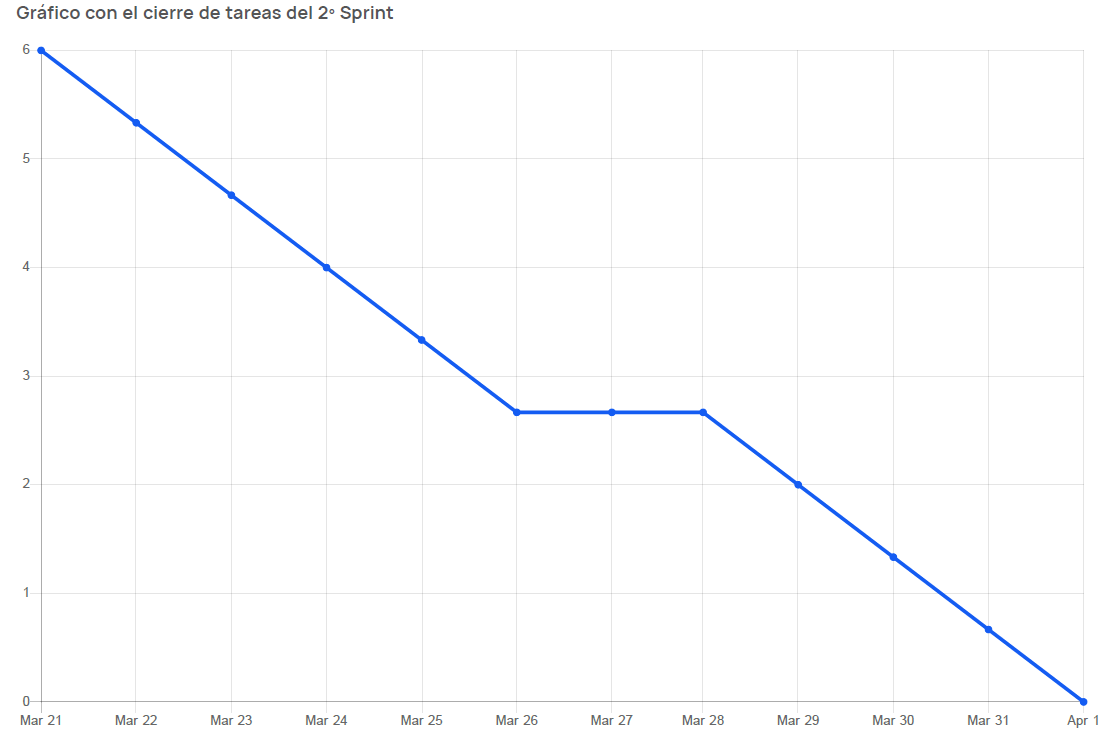
\includegraphics[width=0.6\textwidth]{img/sprint2.PNG}
\caption{Cierre de tareas del SPRINT 2}
\end{figure}
\subsection{\textbf{Sprint 3 (04/04/2022-15/04/2022)}}
Una vez llevada a cabo la conexión de ambas tecnologías, el objetivo era buscar poco a poco la manera de trabajar con el robot a nivel virtual. Para ello, intentaríamos crear un robot virtual a partir de un modelo diseñado que se comporte de maneras similares. 

Las tareas dispuestas para este sprint fueron:
\begin{itemize}
    \item Estudio de la componente\cite{Componentes} Transform de Unity, enfatizando en la rotación y sus valores.
    \item Creación de nueva escena para la replicación virtual de la pinza del robot.
    \item Implementación de métodos: \begin{enumerate}
        \item Get y Set de la posción en el espacio tridimensional.
        \item Get y Set de la apertura de la pinza.
        \item Movimiento en el espacio dada una velocidad lineal y una posición objetivo.
        \item Movimiento que controla la apertura de pinza dada una velocidad de apertura y una apertura objetivo.
    \end{enumerate}
    \item Unificar rotación de cada brazo de la pinza para abrir y cerrar de manera correcta.
    \item Ejecución de pruebas para comprobar el funcionamiento.
\end{itemize}

En este sprint he visto clave el tener que conocer a fondo la manera en la que funcionan las rotaciones dentro de este motor gráfico, ya que tuve alguna complicación a la hora de gestionar estos aspectos en el proyecto.
\begin{figure}[h]
\centering
\label{Cierre de tareas del SPRINT 3}
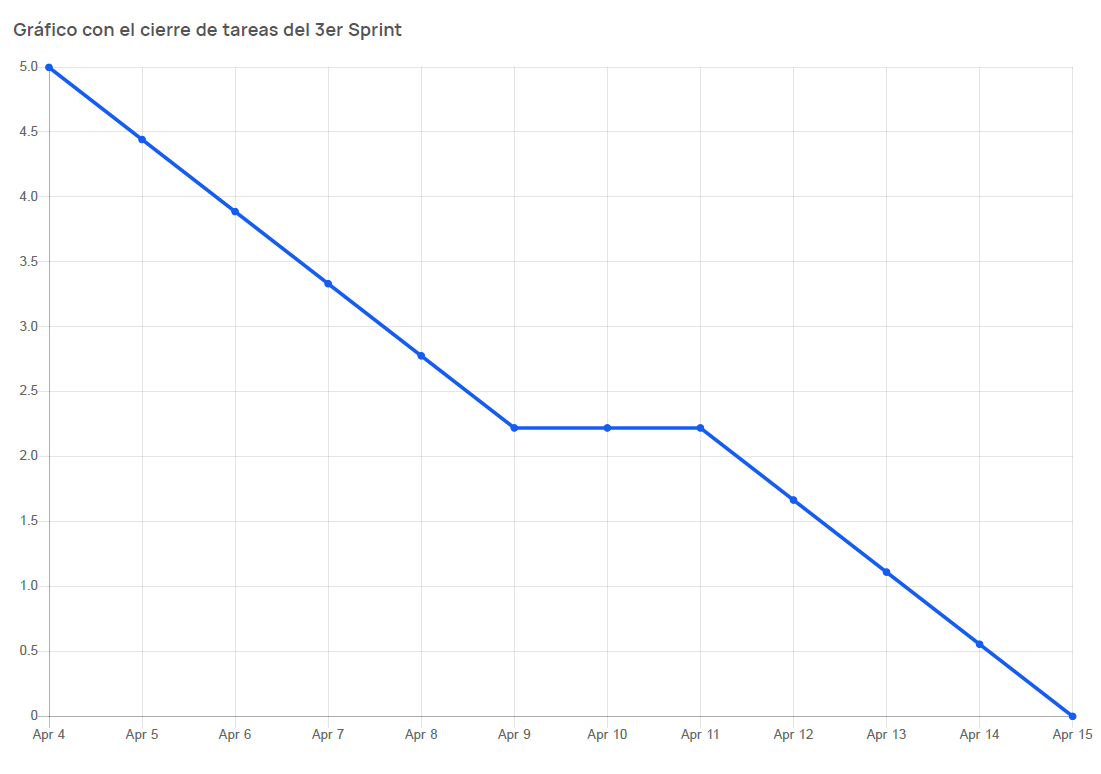
\includegraphics[width=0.6\textwidth]{img/sprint3.PNG}
\caption{Cierre de tareas del SPRINT 3}
\end{figure}
\subsection{\textbf{Sprint 4 (18/04/2022-29/04/2022)}}
El objetivo de llevar a cabo la implementación de los métodos descritos en el anterior sprint en un script, era para poder dotar a la pinza de funciones reales como si fuera el robot. De esta manera, en este sprint el objetivo buscado era fusionar tanto la replicación virtual del robot con la tecnología de los guantes y las gafas desarrollada en el segundo sprint.

Las tareas seleccionadas para este sprint fueron:
\begin{itemize}
    \item Mejorar la automatización de la apertura y cierre de la pinza.
    \item Creación de nueva escena donde serán apreciados los resultados.
    \item Adaptación de la escena de la pinza a esta nueva mediante realidad virtual\cite{VR}
    \item Mostrar virtualmente la representación de las manos en la escena.
    \item Diseñar idea que permita conectar los guantes y la pinza.
    \item Desarrollo del script conector que \begin{enumerate}
        \item Desplace la pinza a una posición cercana de las manos a una velocidad dada.
        \item Abra o cierre la pinza simulada en función de la apertura de nuestro dedo índice y pulgar, dada una velocidad.
    \end{enumerate}
    \item Fusionar todos los puntos en la escena.
    \item Ejecutar pruebas de desplazamiento y apertura para comprobar el correcto funcionamiento.
\end{itemize}

\begin{figure}[h]
\centering
\label{Cierre de tareas del SPRINT 4}
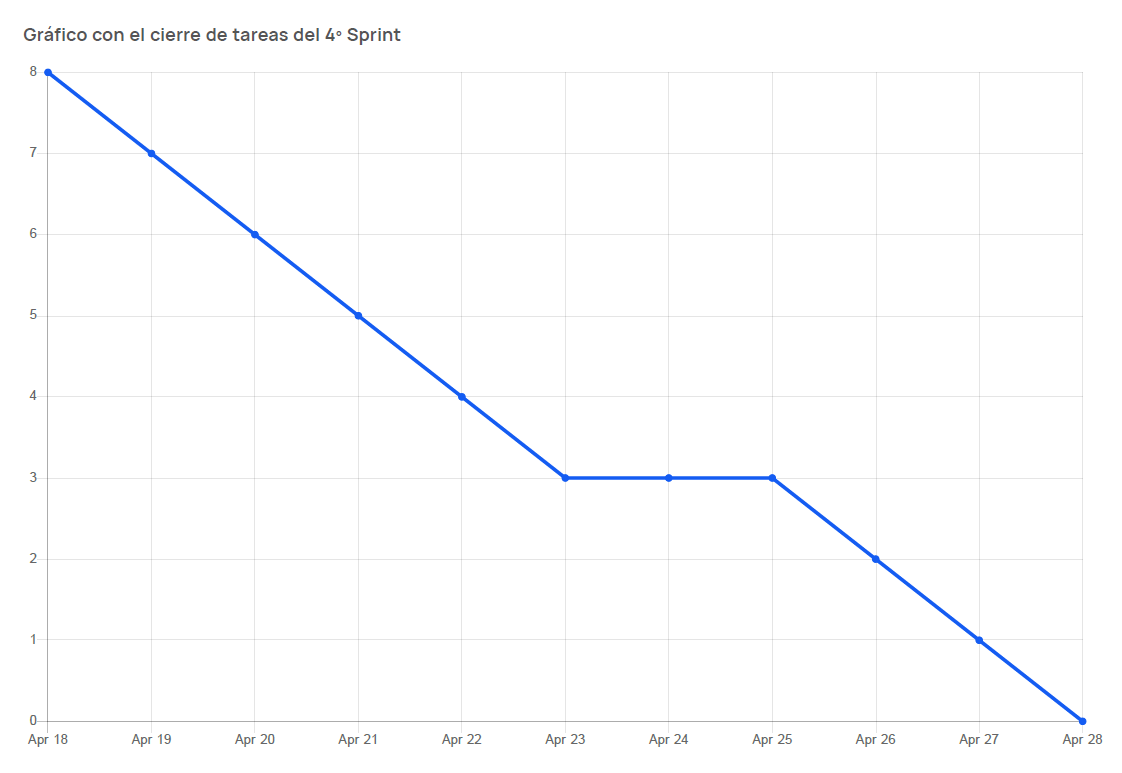
\includegraphics[width=0.6\textwidth]{img/sprint4.PNG}
\caption{Cierre de tareas del SPRINT 4}
\end{figure}
\subsection{\textbf{Sprint 5 (02/05/2022-13/05/2022)}}
Este sprint estaba pensado para comenzar a trabajar con el robot real, ya buscando resultados que den valor a lo realizado durante el proyecto. De esta manera tanto este como el siguiente sprint se antojan como unos de los más complicados, ya que nunca había trabajado con robots previamente a este proyecto.

Los objetivos marcados para cumplir este sprint vienen dados por la consecución de las siguientes tareas:
\begin{itemize}
    \item Investigación y recopilación de información sobre el brazo robótico Kinova
    \item Estudio breve a modo de introducción de ROS \cite{ROS}
    \item Establecer conexión correcta con el robot.
    \item Acceder al robot y a ROS para buscar la lista de topics(funciones) disponibles.
    \item Ejecución de pruebas con el brazo robótico desde otro proyecto.
    \item Parametrización de valores y datos necesarios.
    \item Desarrollo de una nueva escena de conexión con ROS y el robot desde Unity.
    \item Desarrollar un script que permita desplazar la pinza del robot en el espacio.
\end{itemize}

A la correcta consecución de las tareas de este sprint comenzamos a ver poco a poco cual sería el funcionamiento finalmente del robot. 


\begin{figure}[h]
\centering
\label{Cierre de tareas del SPRINT 5}
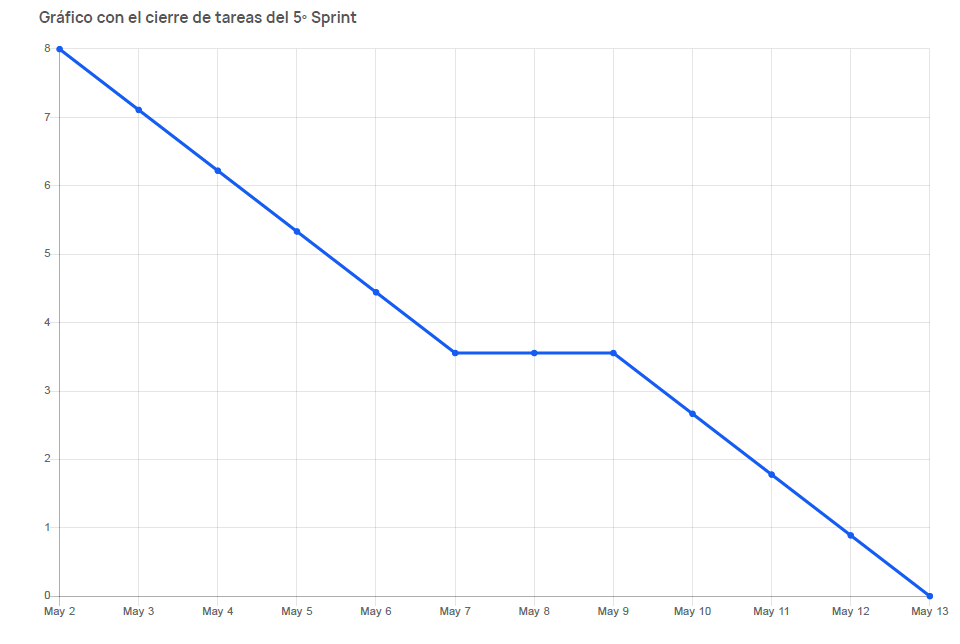
\includegraphics[width=0.6\textwidth]{img/sprint5.PNG}
\caption{Cierre de tareas del SPRINT 5}
\end{figure}
\subsection{\textbf{Sprint 6 (16/05/2022-27/05/2022)}}
Llegados al último sprint dispuesto para el proyecto, nos encontramos muy cerca de los resultados finales deseados. Por ello para este final sprint nos encargaremos de pulir algunos problemas y finalmente dejar perfilada la resolución del proyecto. En la consecución de este sprint encontraremos también la resolución positiva de los objetivos principales de proyecto marcados.

Aquí al acabar este sprint quedarían fusionadas todas las partes y tecnologías tanto vistas, como utilizadas dando lugar al resultado final.

Para finalizar el proyecto de una manera positiva y que se asemeje a lo trazado al comenzar el proyecto deberíamos cumplir las siguientes tareas:
\begin{itemize}
    \item Desarrollo de script que linkee nuestra mano con la pinza del robot y el desplazamiento en el espacio.
    \item Implementación y sincronización de rotación de la pinza con rotación de la mano.
    \item Diseño y desarrollo de un script que gestione la apertura y cierre de la pinza del robot.
    \item Limitar y gestionar valores relativos a la posición para una satisfactoria experiencia del usuario.
    \item Establecer un comando para regreso a posición 'home' para el robot.
    \item Desarrollo de la escena final donde utilizar todo lo llevado a cabo en el proyecto
    \item Ejecución de pruebas de funcionamiento.
    \item Ejecución de pruebas con desplazamiento de objetos.
    \item Filmación de vídeos que muestren el funcionamiento de lo realizado.
\end{itemize}
\newpage
\begin{figure}[h]
\centering
\label{Cierre de tareas del SPRINT 6}
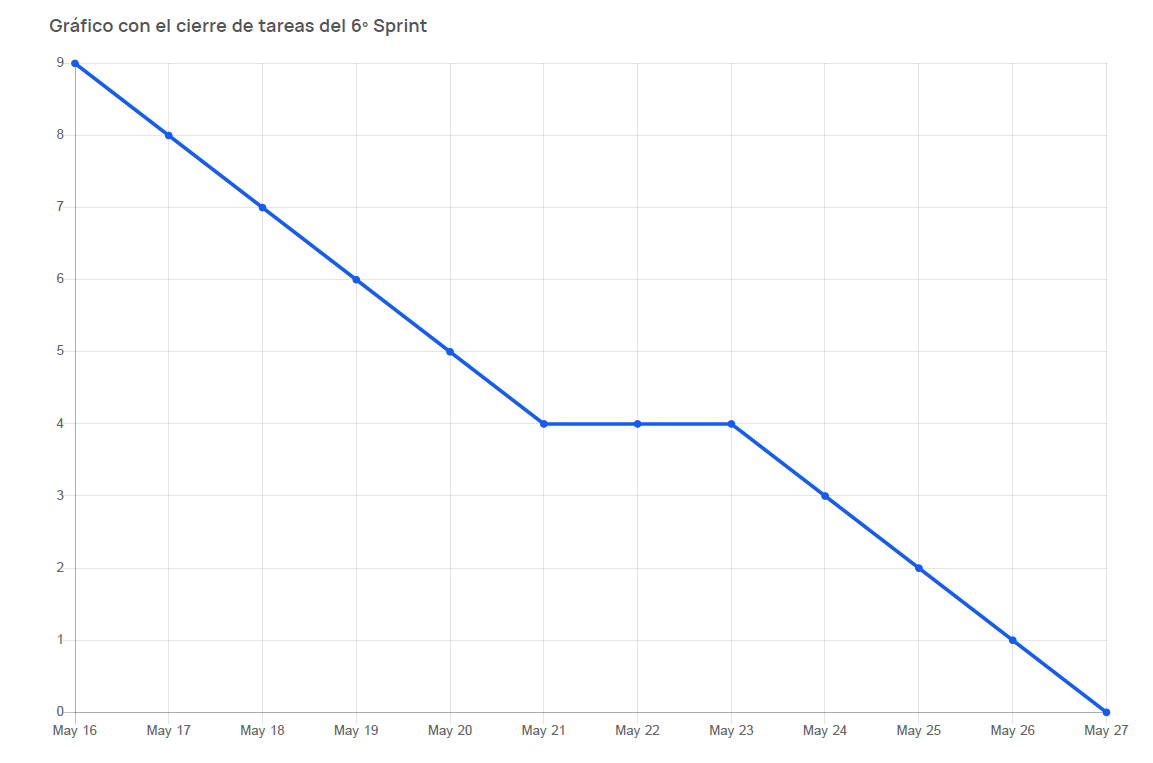
\includegraphics[width=0.6\textwidth]{img/sprint6.PNG}
\caption{Cierre de tareas del SPRINT 6}
\end{figure}
\subsection{\textbf{Final de Proyecto}}
Llegados a la última semana dentro de ITCL\cite{itcl}(30/05/2022-03/06/2022) podemos asegurar que todos los objetivos principales dispuestos han sido cumplidos correctamente, además varios de los secundarios también.

Cabe destacar que la manera de dividir las tareas y organizar el trabajo dentro del proyecto ha sido una de las cosas que ha permitido el ir consiguiendo los objetivos marcados en el tiempo marcado.

A partir de este punto el objetivo que me marco en este sprint 'personal' es el de continuar con la generación de documentación con la herramienta Overleaf, con \LaTeX que ya había ido desarrollando en paralelo con la parte de software del proyecto. De gran ayuda es para el desarrollo de esta documentación el haber ido labrando un documento a modo de diario que iba cumplimentando todas las semanas con lo hecho en esos días.

La entrega y final de esta etapa de TFG finaliza el próximo 13 de Junio de 2022 y hasta entonces el tiempo está dedicado a preparar toda la documentación, anexos y entregables.

\newpage

\section{Estudio de viabilidad}

\subsection{Viabilidad económica}
Uno de los aspectos más importantes a la hora de llevar a cabo el desarrollo de un proyecto es el de controlar los costes y derivados del mismo.

Es por ello que en este apartado dentro del anexo veremos y analizaremos estos costes. Para ello y con vista de que sea más fácil de comprender y desarrollar, dividiremos los costes totales en tres claramente diferenciados: \begin{enumerate}
    \item Coste a nivel \textbf{Hardware} 
    \item Coste a nivel \textbf{Software}
    \item Coste a nivel de \textbf{Personal}
\end{enumerate}

\newpage
\subsubsection{Coste a nivel Hardware}
Dentro de nuestro proyecto algo que juega un papel fundamental es la parte tecnológica, relacionada tanto con la tecnología de realidad virtual\cite{VR} como con la robótica\cite{Robotica} y el ordenador utilizado. Esta parte tiene un determinado coste a nivel de hardware, ya que el utilizado en el proyecto es sofisticado y especializado, que podríamos considerar por encima de lo común.

A continuación se muestra una tabla donde podemos ver tanto el nombre del producto, como el coste propio del producto y la amortización, estableciendo una amortización de cinco años y un uso de tres meses del producto.

\begin{table}[h]
    \centering
    \begin{tabular}{c| c |c}
    \hline
        Producto & Coste & Amortización \\ \hline
        SenseGlove Nova & 4499€ & 899,8€ \\
        Oculus Quest 2 & 350€ & 70€ \\
        Robot Kinova & 20.000€ & 4000€  \\
        Ordenador ITCL & 750€ & 150€ \\ \hline
        \textbf{Total} & 25.599€ & 5119,8€ \\ \hline
    \end{tabular}
    \caption{Coste a nivel Hardware}
    \label{Coste a nivel Hardware}
\end{table}

\subsubsection{Coste a nivel Software}
Otro de los aspectos que tiene vital importancia a la hora de desarrollar software es el coste específico de todos aquellos programas o licencias necesarias para llevar a cabo el desarrollo. Es por ello que a continuación vemos una tabla con el coste de software o de las licencias, considerando dos años de amortización.

\begin{table}[h]
    \centering
    \begin{tabular}{c|c|c}
    \hline
        Producto & Coste & Amortización \\ \hline
         Windows 10 Pro & 259€ & 129,5€ \\ 
         Unity Student & 0€ & 0€ \\ 
         JetBrains Rider (Student) & 0€ & 0€ \\ 
         Overleaf(\LaTeX) University & 0€ & 0€ \\ \hline
         \textbf{Total} & 259€ & 129,5€ \\ \hline
    \end{tabular}
    \caption{Coste a nivel Software}
    \label{Coste a nivel Software}
\end{table}

\subsubsection{Coste a nivel de Personal}
El último aspecto que queda por cubrir a nivel de costes es el destinado al pago del sueldo de los integrantes del personal. En este caso un único desarrollador que ha trabajado durante 300 horas dispersadas en 12 semanas, considerando un sueldo de 25000€ anuales brutos(19.880€ netos), el coste de personal sería: 

\begin{table}[h]
    \centering
    \begin{tabular}{c|c}
    \hline
        Concepto de pago & Coste  \\ \hline
       Retención por IRPF	& 333.91€ \\
       Cuota a la Seg. Social	& 147,17€ \\
       Sueldo neto mensual (12 pagas)  &  1.602,5€ \\
       Coste mensual trabajador & 2083,58€ \\ \hline
       \textbf{Coste total 12 semanas} & \textbf{6250,74€}\\ \hline
    \end{tabular}
    \caption{Costes de Personal}
    \label{Costes de Personal}
\end{table}
Estos costes se han trazado siguiendo un porcentaje de retención de IRPF del 16,03\% y una cuota de seguridad social del 28,3\%.

\subsubsection{Costes Totales}
\begin{table}[h]
    \centering
    \begin{tabular}{c|c}
       \hline Tipo Gasto & Coste  \\ \hline
         Hardware & 25.599€ \\
         Software & 129,5€ \\
         Personal & 6250,74€ \\ \hline
         \textbf{Total} & \textbf{31.979,24€} \\ \hline
    \end{tabular}
    \caption{Costes Totales}
    \label{Costes Totales}
\end{table}



